%
% riemann.tex
%
% (c) 2020 Prof Dr Andreas Müller, Hochschule Rapperswil
%
\begin{frame}
\frametitle{Integral}
\vspace{-20pt}
\begin{columns}[t]
\begin{column}{0.51\hsize}
\begin{block}{Aufgabe}
Für $f\colon[a,b]\to\mathbb R$ stetig berechne
\vspace{-5pt}
\[
I = \int_a^b f(x)\,dx
\]
\end{block}
\vspace{-15pt}
\uncover<2->{%
\begin{block}{Interpretationen}
\begin{itemize}
\item<3-> Fläche unter der Kurve
\item<6-> Stammfunktion $F(x)$ mit $F'(x)=f(x)$
$\Rightarrow$
$I = F(b)-F(a)$
\item<7->
Lösung $y(x)$ der Differentialgleichung%
\vspace{-5pt}
\begin{align*}
y' &= f(x),&y(a)&=0\\[-20pt]
\end{align*}
$\Rightarrow$ $I = y(b)$
\end{itemize}
\end{block}}
\end{column}
\begin{column}{0.44\hsize}
\begin{center}
\uncover<4->{%
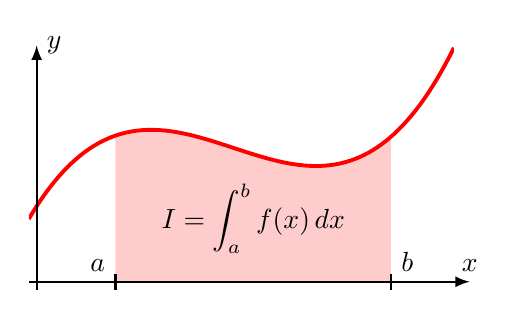
\begin{tikzpicture}[>=latex,thick]
\uncover<5->{
\fill[color=red!20]
	(4.5,0)--
	(1.0,0)--
	plot[domain=1.0:4.5,samples=100]
	({\x},{0.1*(\x-0.2)*(\x-2.5)*(\x-4.8)+1.2+0.2*\x})--cycle;
}
\begin{scope}
\clip (-0.1,0) rectangle (5.3,3);
\draw[color=red,line width=1.4pt] plot[domain=-0.1:5.3,samples=100]
	({\x},{0.1*(\x-0.2)*(\x-2.5)*(\x-4.8)+1.2+0.2*\x});
\uncover<5->{
\node at (2.75,0.8) {$\displaystyle I=\int_a^bf(x)\,dx$};
}
\end{scope}
\draw[->] (-0.1,0)--(5.5,0) coordinate[label={$x$}];
\draw[->] (0,-0.1)--(0,3.0) coordinate[label={right:$y$}];
\draw (1,-0.1)--(1,0.1);
\node at (1,0) [above left] {$a$};
\draw (4.5,-0.1)--(4.5,0.1);
\node at (4.5,0) [above right] {$b$};
\end{tikzpicture}}
\uncover<8->{%
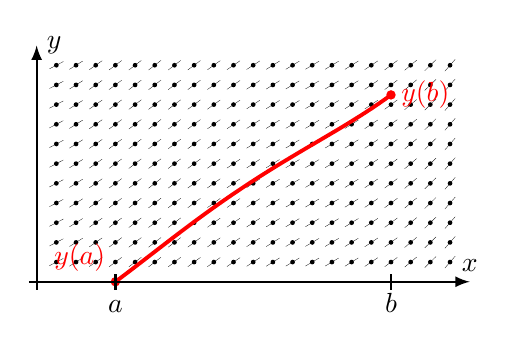
\begin{tikzpicture}[>=latex,thick]
\uncover<8->{
\foreach \x in {0.25,0.5,...,5.25}{
	\foreach \y in {0.25,0.5,...,2.8}{
		\fill ({\x},{\y}) circle[radius=0.03];
		\pgfmathparse{atan(0.4*(0.1*(\x-0.2)*(\x-2.5)*(\x-4.8)+1.2+0.2*\x))}
		\xdef\m{\pgfmathresult}
		\draw[line width=0.1pt]
			({\x-0.1*cos(\m)},{\y-0.1*sin(\m)})
			--
			({\x+0.1*cos(\m)},{\y+0.1*sin(\m)});
	}
}
}
\xdef\x{1}
\pgfmathparse{(((0.025*\x-0.25)*\x+0.773)*\x+0.96)*\x}
\xdef\Fa{\pgfmathresult}
\xdef\x{4.5}
\pgfmathparse{(((0.025*\x-0.25)*\x+0.773)*\x+0.96)*\x-\Fa}
\xdef\Fb{\pgfmathresult}
\pgfmathparse{((0.025*\x-0.25)*\x+0.773)*\x+0.96}
\uncover<9->{
\draw[color=red,line width=1.4pt]
	plot[domain=1:4.5,samples=100]
		({\x},{0.4*((((0.025*\x-0.25)*\x+0.773)*\x+0.96)*\x-\Fa)});
\fill[color=red] (1,0) circle[radius=0.06];
\fill[color=red] (4.5,{0.4*\Fb}) circle[radius=0.06];
\node[color=red] at (1,0) [above left] {$y(a)$};
\node[color=red] at (4.5,{0.4*\Fb}) [right] {$y(b)$};
}
\draw (1,-0.1)--(1,0.1);
\node at (1,0) [below] {$a\mathstrut$};
\draw (4.5,-0.1)--(4.5,0.1);
\node at (4.5,0) [below] {$b\mathstrut$};
\draw[->] (-0.1,0)--(5.5,0) coordinate[label={$x$}];
\draw[->] (0,-0.1)--(0,3.0) coordinate[label={right:$y$}];
\end{tikzpicture}}
\end{center}
\end{column}
\end{columns}
\end{frame}
